A rainha morreu.

Imediatamente após o falecimento da monarca, o povo começou a
especular não apenas quem será o próximo rei, mas também quem
sentará no trono depois dele, e depois dele, e depois dele, etc. Em pouco tempo, saber toda a linha de sucessão ao
trono se tornou importantíssimo para a população.

Pelas regras da monarquia, o primeiro herdeiro ao trono é o filho mais
velho da rainha. Em seguida, vem os demais filhos da rainha, em ordem decrescente de
idade.

Após todos os filhos diretos da rainha, vem os filhos diretos do filho mais
velho dela. Em seguida, vem os filhos diretos do segundo filho mais velho da
rainha, e assim por diante.

Como exemplo, a figura abaixo apresenta uma possível árvore genealógica da família real,
indicando o ano de nascimento de cada herdeiro da rainha, e sua ordem na linha
de sucessão ao trono:

\begin{center}
    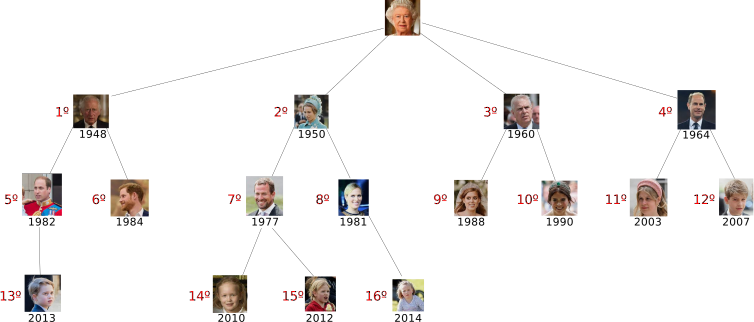
\includegraphics[scale=0.5]{herdeiros/herdeiros.png}
\end{center}

Dada a árvore genealógica da família real e o ano de nascimento de cada
herdeiro, determine toda a linha de sucessão ao trono.

\subsection*{Entrada}

A primeira linha contém um inteiro $N$ ($1 \leq N \leq 10^5$), o número de
herdeiros ao trono. Considere que os herdeiros são numerados de $1$ a $N$.
As próximas $N$ linhas descrevem um herdeiro cada. A linha $i$ $(1 \leq i \leq
        N)$ contém
dois inteiros $P_i$ e $D_i$ ($0 \leq P_i \leq N$, $0 \leq D_i \leq 10^5$), onde $P_i$ é o identificador do pai do herdeiro $i$ (ou 0 caso
o herdeiro $i$ seja filho direto da rainha), e $D_i$ é o ano de nascimento do
herdeiro $i$.

Não haverá dois herdeiros que nasceram no mesmo ano.

\subsection*{Saída}

Imprima $N$ linhas com os identificadores dos herdeiros, um por linha, na ordem
da linha de sucessão ao trono.

\newpage
\begin{table}[!h]
\centering
\begin{tabular}{|l|l|}
\hline
\begin{minipage}[t]{3in}
\textbf{Exemplo de entrada}
\begin{verbatim}
5
0 1961
0 1933
0 1957
0 2022
0 1970
\end{verbatim}
\vspace{1mm}
\end{minipage}
&
\begin{minipage}[t]{3in}
\textbf{Exemplo de saída}
\begin{verbatim}
2
3
1
5
4
\end{verbatim}
\vspace{1mm}
\end{minipage} \\
\hline
\end{tabular}
\end{table}



\begin{table}[!h]
\centering
\begin{tabular}{|l|l|}
\hline
\begin{minipage}[t]{3in}
\textbf{Exemplo de entrada}
\begin{verbatim}
16
2 1990
0 1960
5 1977
13 2014
0 1950
0 1964
9 1984
6 2007
0 1948
15 2013
3 2012
6 2003
5 1981
2 1988
9 1982
3 2010
\end{verbatim}
\vspace{1mm}
\end{minipage}
&
\begin{minipage}[t]{3in}
\textbf{Exemplo de saída}
\begin{verbatim}
9
5
2
6
15
7
3
13
14
1
12
8
10
16
11
4
\end{verbatim}
\vspace{1mm}
\end{minipage} \\
\hline
\end{tabular}
\end{table}
